\subsection{Discontinuous conduction mode}
\label{DCM_Discussion}

\todo{DCM content is here, consider revising location. AT}

According to chapter 5 of "Fundamentals of Power Electronics" \cite{Erickson} "the discontinuous conduction mode (DCM) arises when the switching ripple in an inductor current is large enough to cause the polarity of the applied switch current to reverse". 

In the case of the bidirectional non-inverting buck-boost, the MOSFETs do not stop reverse current flow like diodes would do, this fact makes the system behave in unexpected ways since current can flow through the coil in the opposite direction. An example of this could be found when working in buck mode with a very low power generation at the PV. In this case, since the current is not blocked by a diode, it falls bellow zero, current would then start flowing out of the output capacitor and into M4 through the inductor, charging it in the opposite direction. When MOSFET 1 goes back to ON state, the current would then flow through it and into the input capacitor and the PV. 

The boundaries for entering this DCM scenario are dependent on the PV current $I_{MPP}$ and on the voltage at the output. As the power generated by the PV decreases due to a change on the environmental conditions, the current also drops. Under these circumstances there is a limit for the inductor to work in continuous conduction mode (CCM). If this limit is exceeded, the inductor would undergo negative current.

However, the conditions for the inductor to enter DCM are very exceptional. In the figure \ref{DCM_3D} the inductor distance to reach DCM under different output voltages and generated powers is shown. The power plotted has been calculated at a constant temperature of $15\dec C$ and at changing irradiance from $5W/m^2$ to $100W/m^2$. For this simulation, buck mode is tested and the output voltage values go from $10V$ up to $V_{MPP}$. All the calculations have been performed assuming MPP.
The z-axis of the plot represents the distance from the lower peak of the current ripple to zero.


\begin{figure}[H]
	\begin{center}
	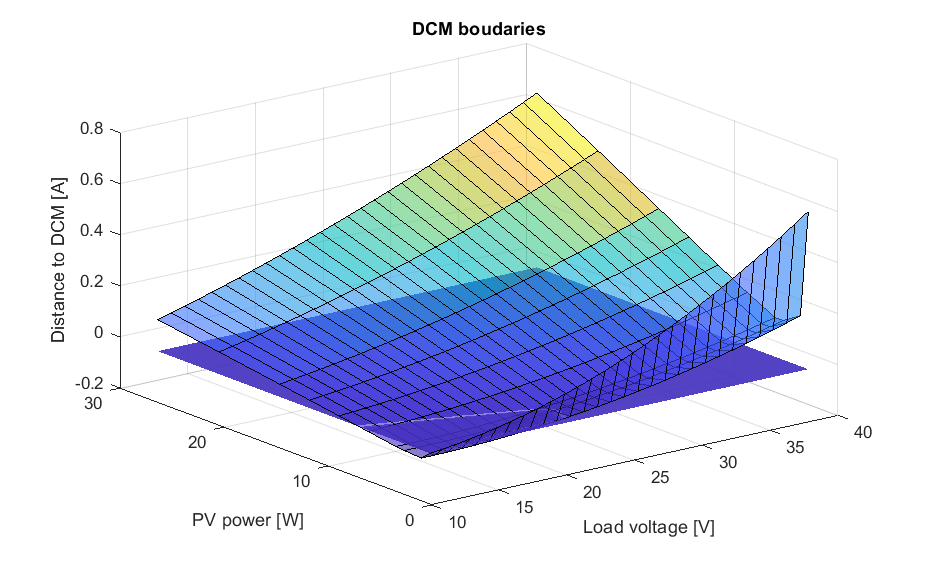
\includegraphics[width=1\textwidth]{../Pictures/DistanceToDCM.png}
		\caption{Boundary conditions for DCM.}
		\label{DCM_3D}
	\end{center}	
\end{figure}

In the figure, it is seen how DCM is only reached under very limited conditions, with very low power being generated in the PV. Due to this, when the behavior is present, the current being generated is very low and it is very unlikely that the PV would be damaged from this issue. Nevertheless, it is a topic of great consideration for further research.


